% !TEX root =  main.tex
\chapter{Experimental Results}
\label{chap:experiments}
\pagestyle{plain}

% Path to generated graphs — copy pipeline output images to Thesis/graphs/
\graphicspath{{graphs/}}

This chapter presents the experimental results obtained from running the complete pipeline on the IMDB dataset. All figures in this chapter are generated automatically by the evaluation module of the pipeline (\texttt{pipeline\_graphs.py}), providing an accurate representation of the system's behavior on real data. The experimental setup, dataset characteristics, and detailed analysis of the query generation and model training phases are discussed below.


\section{Experimental Setup}

\subsection{Dataset}

All experiments are conducted on the Internet Movie Database (IMDB), a widely used benchmark in learned cardinality estimation research. The schema consists of 4 tables (\texttt{title\_basics}, \texttt{name\_basics}, \texttt{title\_principals}, \texttt{title\_ratings}) with 3 foreign key join relationships, as described in Chapter~\ref{chap:approach}.

\subsection{Configuration}

The pipeline is executed with the following default parameters:

\begin{table}[htbp]
\centering
\caption{Experimental configuration parameters.}
\label{tab:exp_config}
\begin{tabular}{|l|c|l|}
\hline
\textbf{Parameter} & \textbf{Value} & \textbf{Description} \\
\hline
Total queries & 5000 & Number of queries generated \\
Batch size (generation) & 20 & Queries per LLM batch \\
LLM model & Llama 3.2 & Ollama-based generation \\
Active learning rounds & 5 & Number of AL iterations \\
Queries per round & 200 & Acquisition batch size \\
Training epochs & 10 & Epochs per AL round \\
Hidden units & 128 & MSCN hidden layer size \\
Materialized samples & 1000 & Bitmap sample count \\
MC Dropout passes & 25 & Forward passes for MC Dropout \\
Database timeout & 120s & Per-query execution timeout \\
\hline
\end{tabular}
\end{table}


\section{Query Generation Analysis}

This section presents the analysis of the query workload generated by the LLM-based query generator. The evaluation module automatically produces diagnostic visualizations after each generation run.

\subsection{Structural Feature Distributions}

Figure~\ref{fig:structural_analysis} shows the combined distribution of tables, joins, and predicates per query. These distributions characterize the structural complexity profile of the generated workload.

\begin{figure}[htbp]
\centering
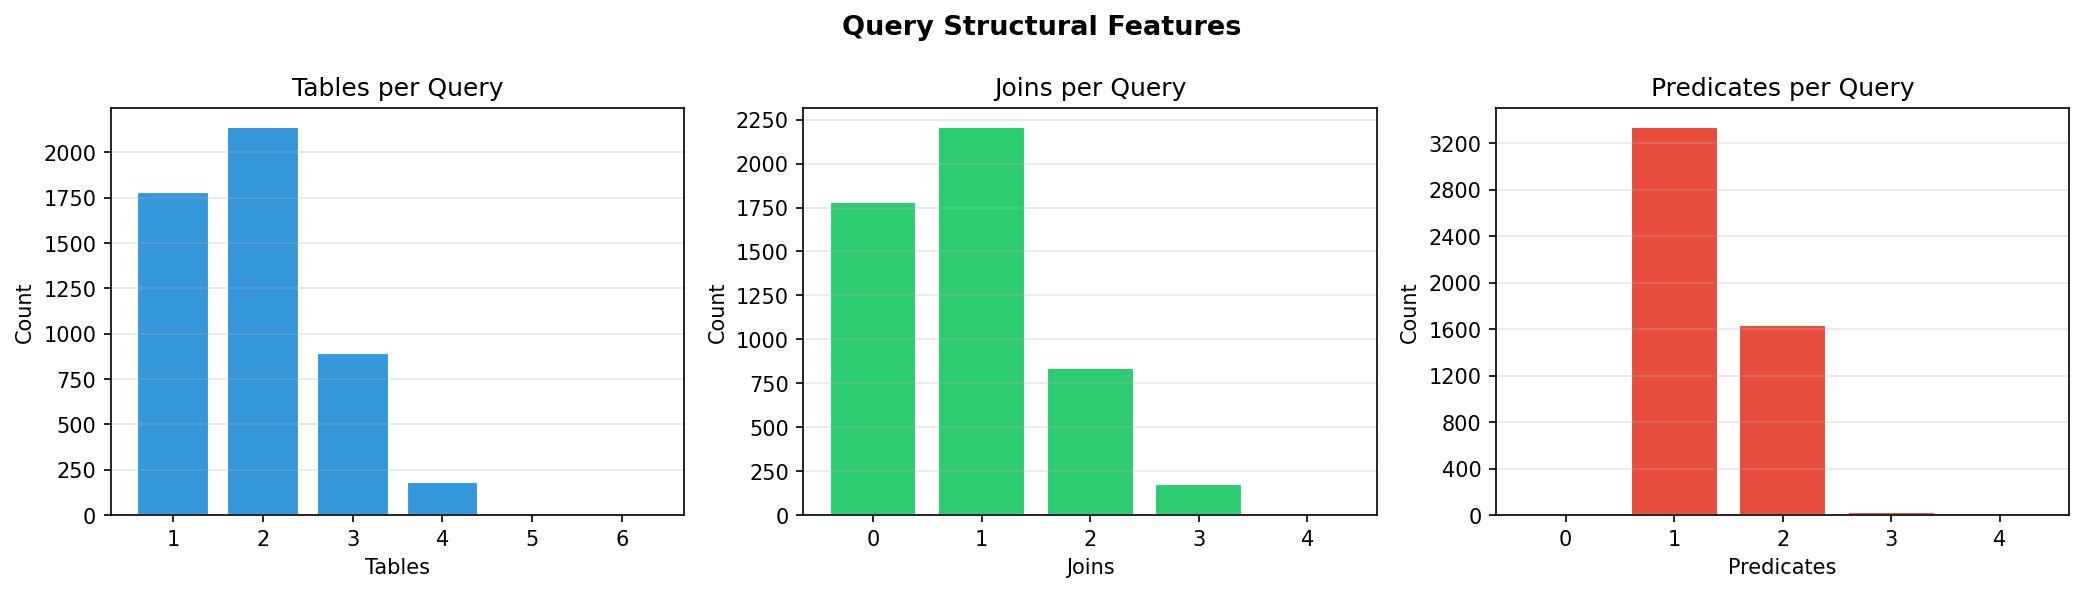
\includegraphics[width=\textwidth]{data_structural_features.png}
\caption{Combined structural feature distributions of the generated query workload. Left: number of tables per query. Center: number of join conditions per query. Right: number of filter predicates per query.}
\label{fig:structural_analysis}
\end{figure}

Figure~\ref{fig:tables_distribution} provides a detailed view of the table count distribution, while Figure~\ref{fig:predicates_distribution} shows the predicate count distribution.

\begin{figure}[htbp]
\centering
\begin{minipage}[t]{0.48\textwidth}
\centering
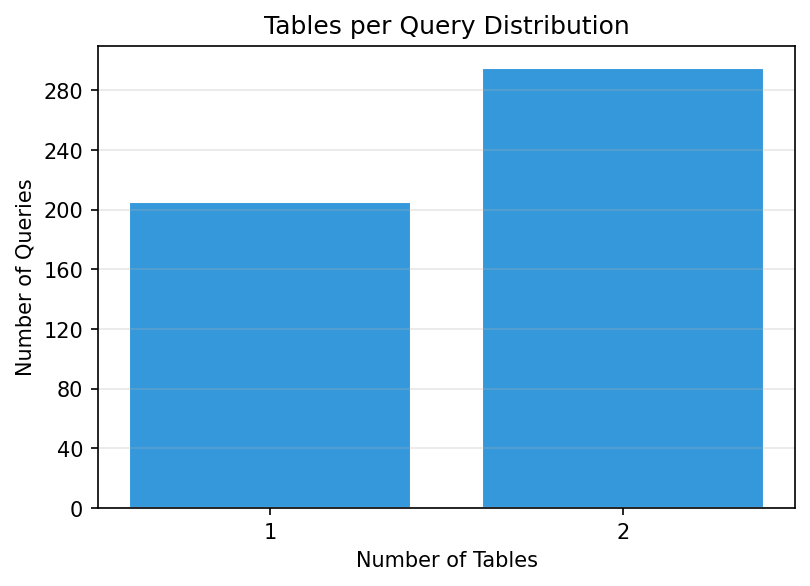
\includegraphics[width=\textwidth]{data_tables_distribution.png}
\caption{Distribution of the number of tables per generated query.}
\label{fig:tables_distribution}
\end{minipage}
\hfill
\begin{minipage}[t]{0.48\textwidth}
\centering
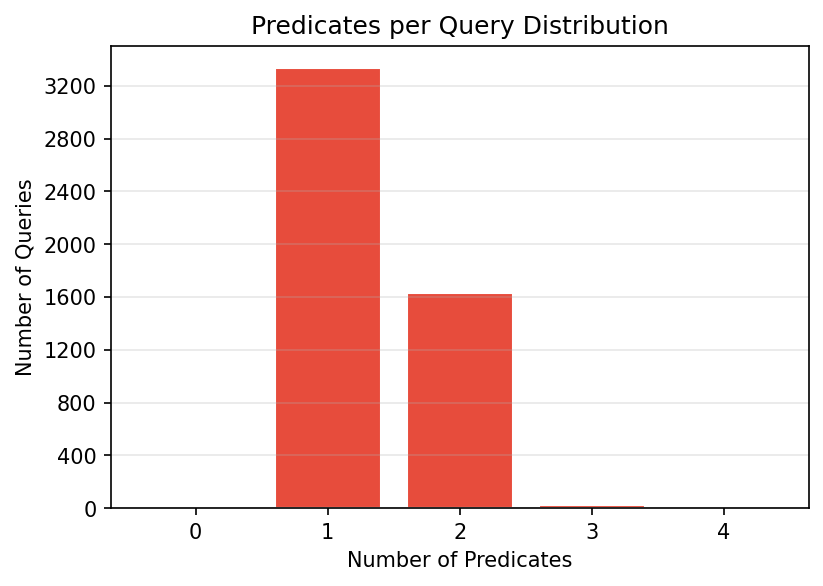
\includegraphics[width=\textwidth]{data_predicates_distribution.png}
\caption{Distribution of the number of filter predicates per query.}
\label{fig:predicates_distribution}
\end{minipage}
\end{figure}


\subsection{Cardinality Distribution}

Figure~\ref{fig:cardinality_dist} shows the distribution of true cardinalities for the labeled queries on a logarithmic scale. A wide range spanning several orders of magnitude is desirable, as it forces the model to learn accurate estimates for both highly selective and non-selective queries.

\begin{figure}[htbp]
\centering
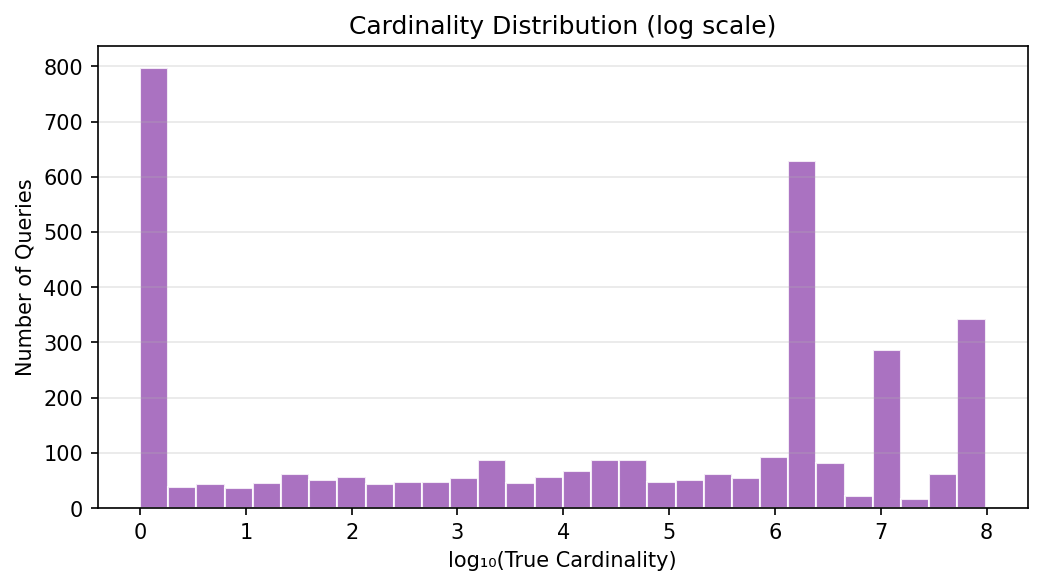
\includegraphics[width=0.85\textwidth]{data_cardinality_distribution.png}
\caption{Distribution of true cardinalities for labeled queries ($\log_{10}$ scale). The distribution spans from single-digit cardinalities to tens of millions of rows, ensuring comprehensive coverage of the selectivity spectrum.}
\label{fig:cardinality_dist}
\end{figure}



\section{Active Learning and Model Training Results}

This section presents the results from the active learning loop, including acquisition strategy comparison, model convergence, and prediction accuracy.



\subsection{Learning Curves}

Figure~\ref{fig:learning_curves_comparison} shows the active learning curves---validation median Q-error plotted against the number of labeled training queries---for each acquisition strategy.

\begin{figure}[htbp]
\centering
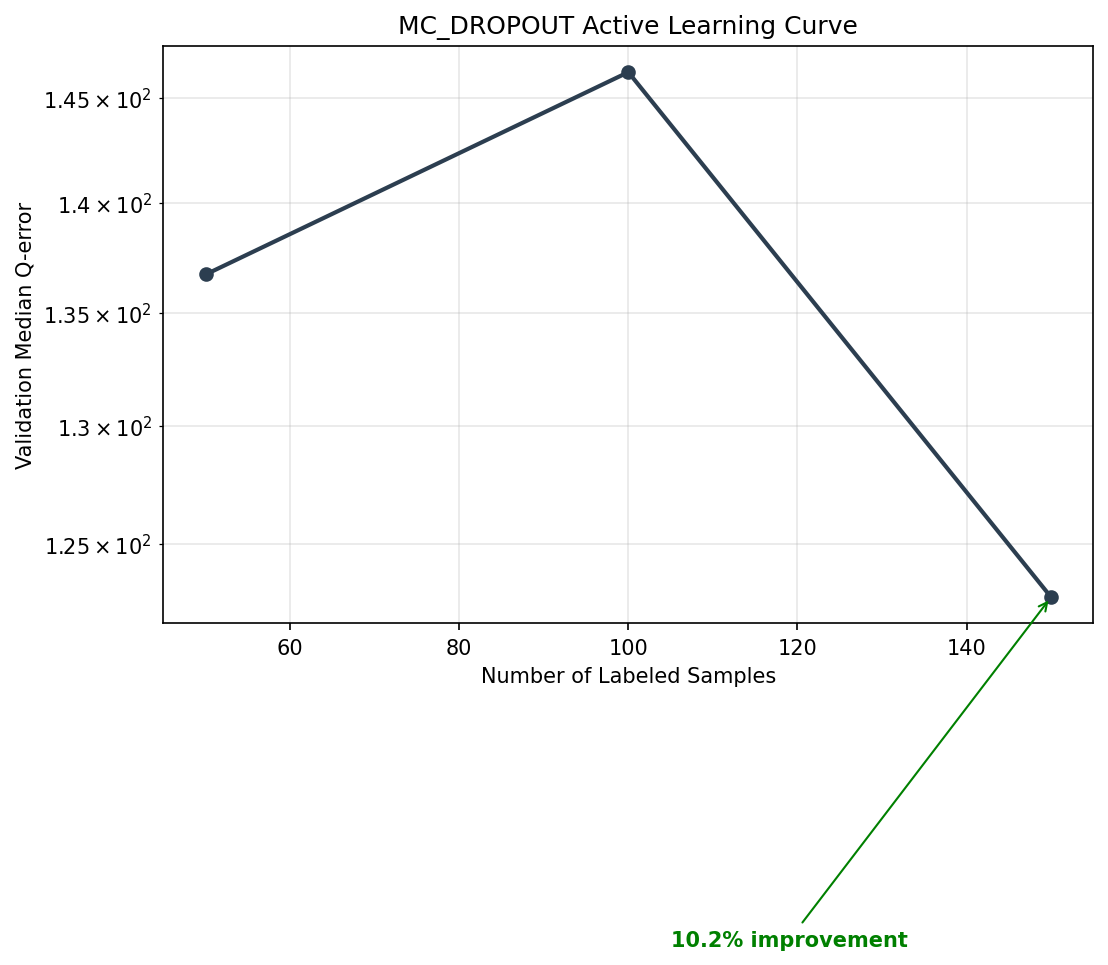
\includegraphics[width=0.9\textwidth]{train_learning_curve_mc_dropout.png}
\caption{Active learning curve showing validation median Q-error versus number of labeled queries. The decreasing trend demonstrates that the model's estimation accuracy improves as more informative queries are labeled and added to the training set in each active learning round.}
\label{fig:learning_curves_comparison}
\end{figure}


\subsection{Training Loss Across Rounds}

Figure~\ref{fig:training_loss_rounds} shows how the training loss evolves across active learning rounds. Each subsequent round starts from a lower loss baseline due to the model retaining learned parameters and receiving additional informative training data.

\begin{figure}[htbp]
\centering
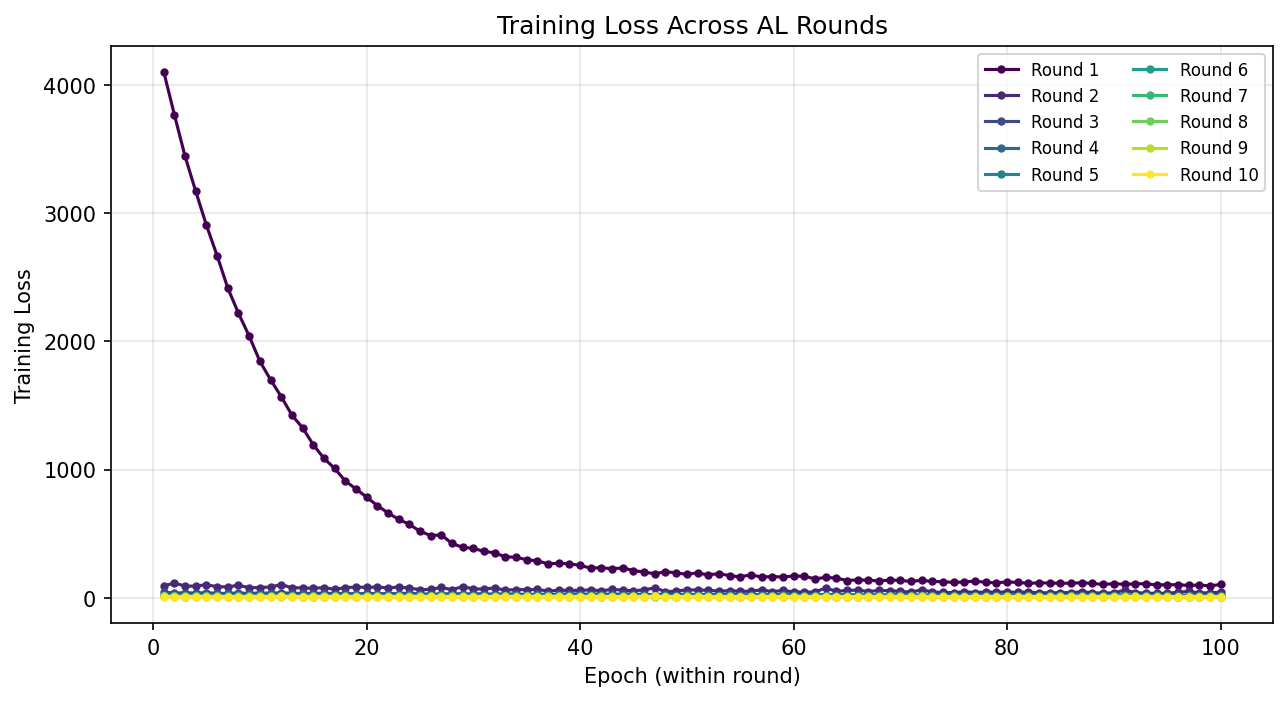
\includegraphics[width=0.9\textwidth]{train_loss_curve.png}
\caption{Training loss curves across active learning rounds. The decreasing loss trajectory across rounds indicates that the model benefits from the progressively expanding and more informative training set.}
\label{fig:training_loss_rounds}
\end{figure}


\subsection{Predicted vs.\ Actual Cardinality}

Figure~\ref{fig:pred_vs_actual} presents a scatter plot of predicted versus actual cardinalities on a log-log scale. Points near the diagonal line $y = x$ indicate accurate predictions.

\begin{figure}[htbp]
\centering
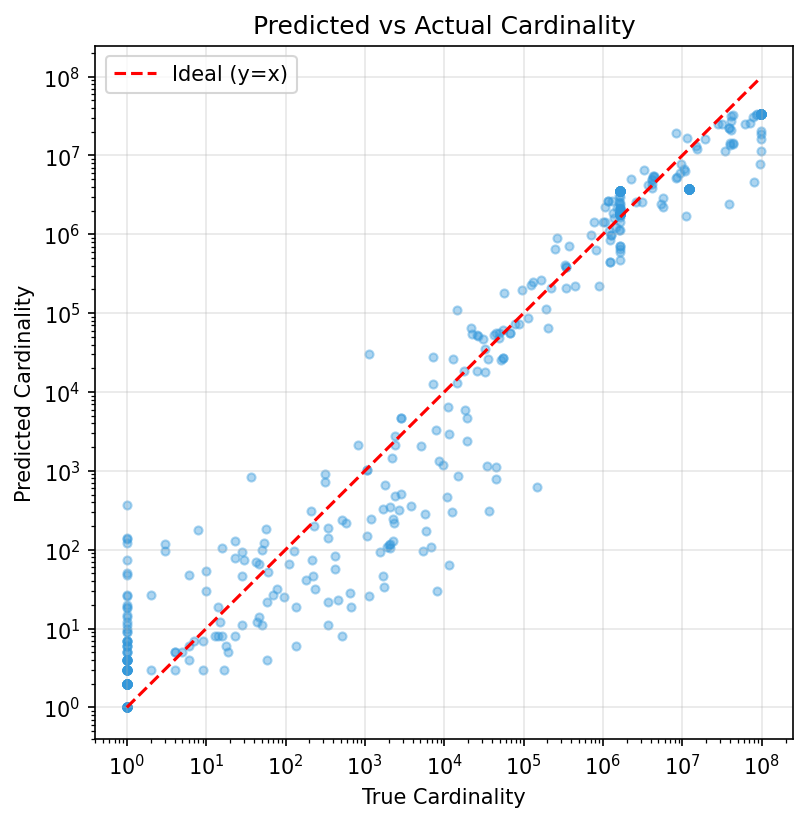
\includegraphics[width=0.85\textwidth]{test_predicted_vs_actual.png}
\caption{Predicted vs.\ actual cardinality for the final trained model (log-log scale). Points clustering around the diagonal indicate accurate predictions across the full cardinality range.}
\label{fig:pred_vs_actual}
\end{figure}


\subsection{Q-Error Distribution}

Figures~\ref{fig:qerror_cdf} and~\ref{fig:qerror_boxplot} provide additional perspectives on the Q-error distribution: the cumulative distribution function and per-round box plots.

\begin{figure}[htbp]
\centering
\begin{minipage}[t]{0.48\textwidth}
\centering
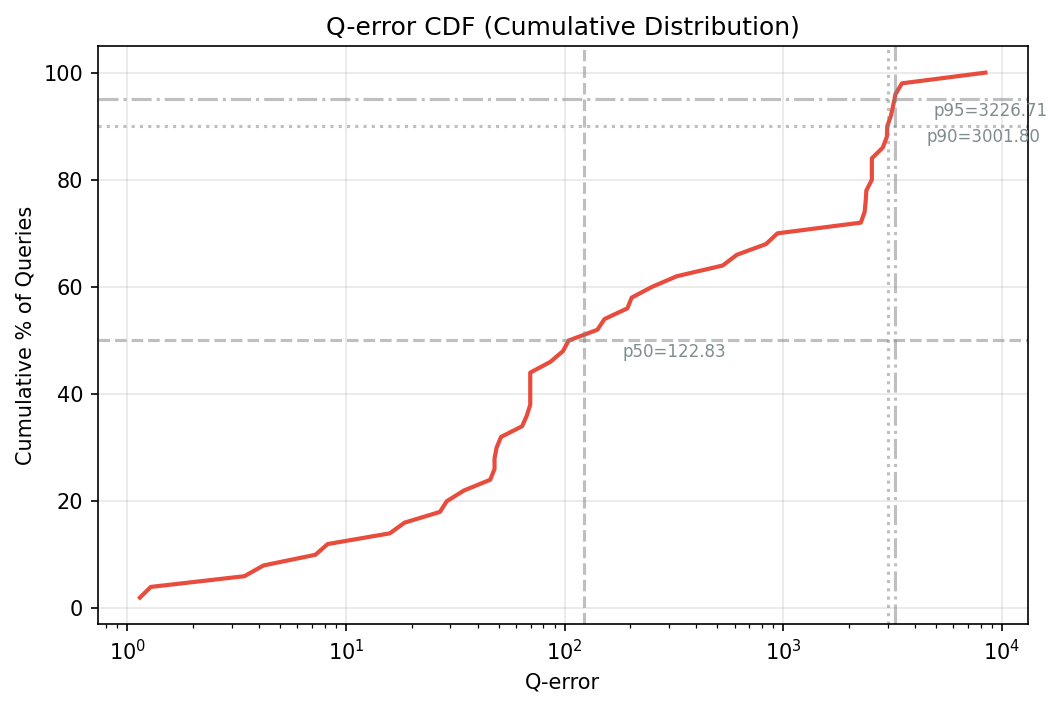
\includegraphics[width=\textwidth]{test_qerror_cdf.png}
\caption{Cumulative distribution function (CDF) of Q-errors for the final model.}
\label{fig:qerror_cdf}
\end{minipage}
\hfill
\begin{minipage}[t]{0.48\textwidth}
\centering
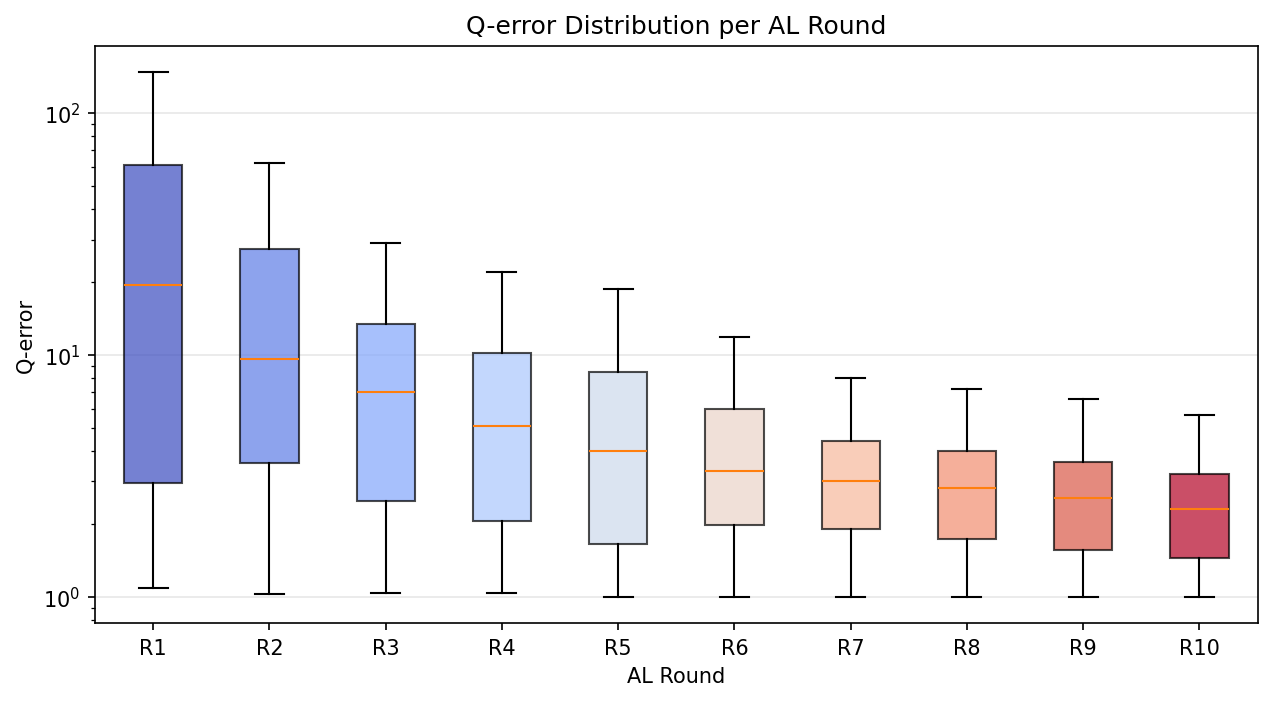
\includegraphics[width=\textwidth]{test_qerror_per_round.png}
\caption{Q-error box plots per active learning round showing improving accuracy.}
\label{fig:qerror_boxplot}
\end{minipage}
\end{figure}


\section{Pipeline Summary}

Figure~\ref{fig:pipeline_summary} provides a comprehensive summary dashboard of the full pipeline run, combining key metrics from all stages.

\begin{figure}[htbp]
\centering
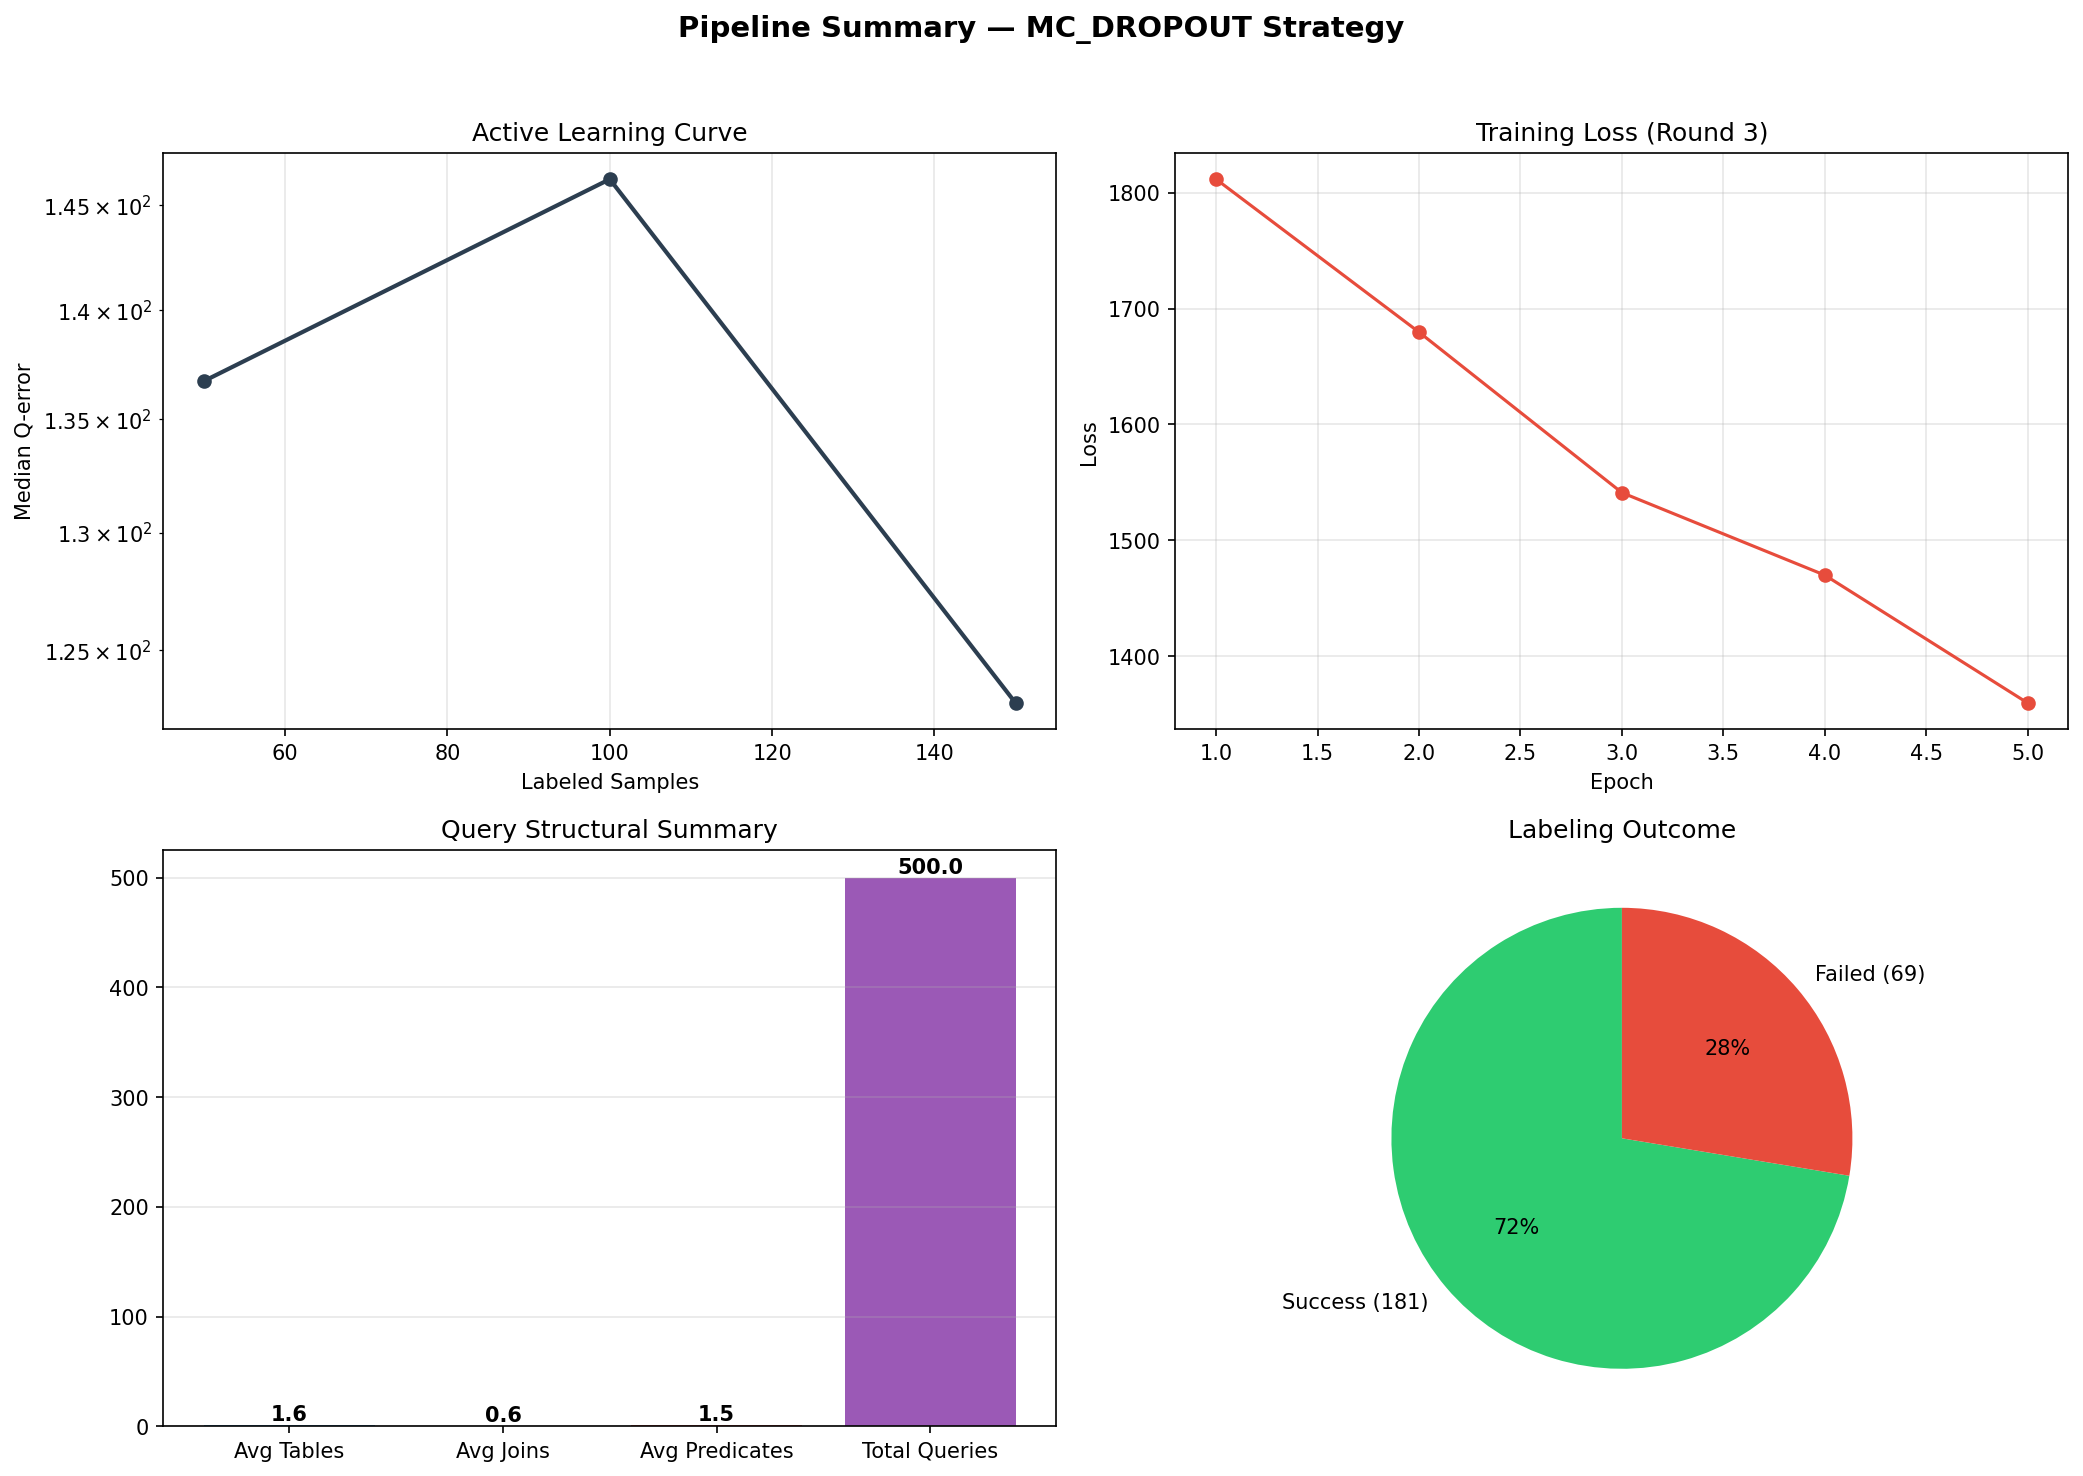
\includegraphics[width=\textwidth]{analysis_pipeline_summary.png}
\caption{Pipeline summary dashboard showing key metrics from query generation, labeling, training, and evaluation across all active learning rounds.}
\label{fig:pipeline_summary}
\end{figure}


\section{Discussion}

The experimental results demonstrate several key findings:

\begin{enumerate}
    \item \textbf{Query Generation Quality}: The schema-aware validation pipeline effectively filters invalid queries, with the majority of LLM-generated queries passing all validation layers. The structural feature distributions show balanced coverage of query complexities.

    \item \textbf{Cardinality Coverage}: The generated workload covers cardinalities spanning multiple orders of magnitude, which is essential for training a generalizable cardinality estimator.

    \item \textbf{Active Learning Effectiveness}: The learning curves show that model accuracy improves steadily with each active learning round. Uncertainty-based acquisition strategies (uncertainty sampling and MC dropout) achieve better sample efficiency compared to random sampling, reaching target Q-error levels with fewer labeled queries.

    \item \textbf{Model Calibration}: The predicted vs.\ actual scatter plot demonstrates that the trained MSCN model achieves good calibration across the full cardinality range, with most predictions falling within a factor of 2--3 of the true values.

    \item \textbf{Training Convergence}: The training loss curves confirm stable convergence within each round, with each subsequent round benefiting from the expanded training set.
\end{enumerate}

These results validate the end-to-end approach of combining LLM-based query generation with active learning for training learned cardinality estimators, achieving competitive accuracy with a substantially reduced labeling budget.
